\documentclass[12pt]{article}

\usepackage[margin=1in]{geometry} 
\usepackage{amsmath,amsthm,amssymb}
\usepackage[spanish]{babel}
\usepackage[utf8]{inputenc}
\usepackage{tikz-cd}
\usepackage{amsmath}
\usepackage[shortlabels]{enumitem}
\usepackage{mathtools}
\usepackage{float}
\usepackage{listings}
\usepackage{xcolor}


\graphicspath{{img/}}

\title{SWAP: Práctica 4}
\author{
        Antonio Gámiz Delgado
}

\begin{document}
\maketitle

\section{Generar e instalar un certificado autofirmado }

Activamos el módulo SSL de Apache, generamos los certificados indicándole la ruta donde queremos que se generen:

\begin{figure}[H]
\center
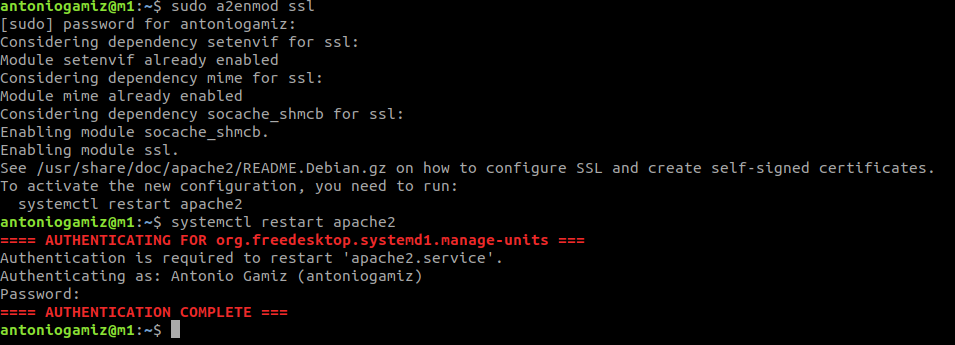
\includegraphics[scale=0.5]{1.png}
\caption{Módulo SSL de Apache}
\end{figure}
\begin{figure}[H]
\center
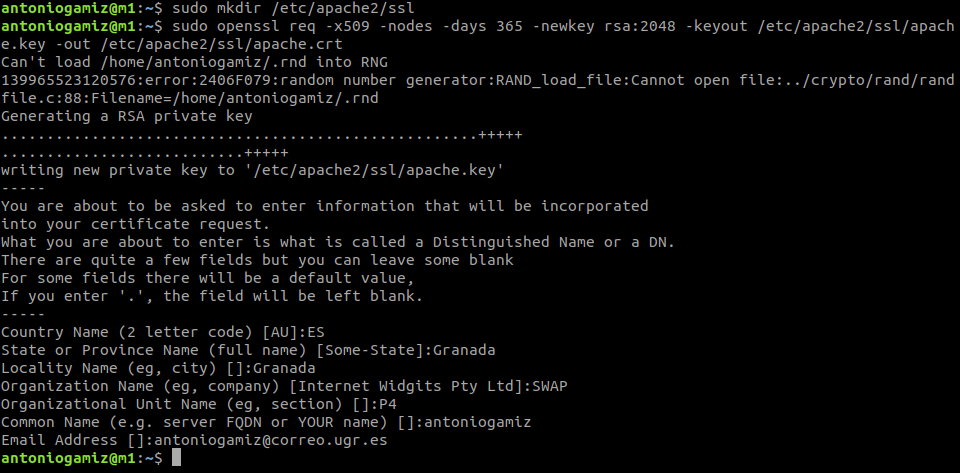
\includegraphics[scale=0.5]{2.png}
\caption{Generación de los certificados}
\end{figure}

\begin{figure}[H]
\center
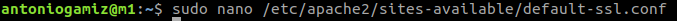
\includegraphics[scale=0.5]{3.png}
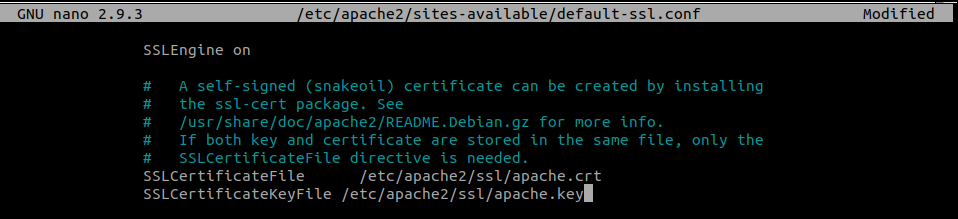
\includegraphics[scale=0.5]{4.png}
\caption{Indicamos a Apache donde se encuentran nuestros certificados}
\end{figure}

Activamos el sitio \textit{default-ssl} y reiniciamos Apache:
\begin{figure}[H]
\center
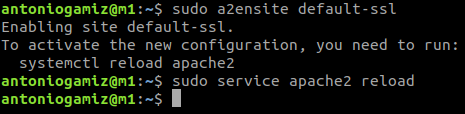
\includegraphics[scale=0.5]{5.png}
\end{figure}

Comprobamos que efectivamente el certificado no es válido:

\begin{figure}[H]
\center
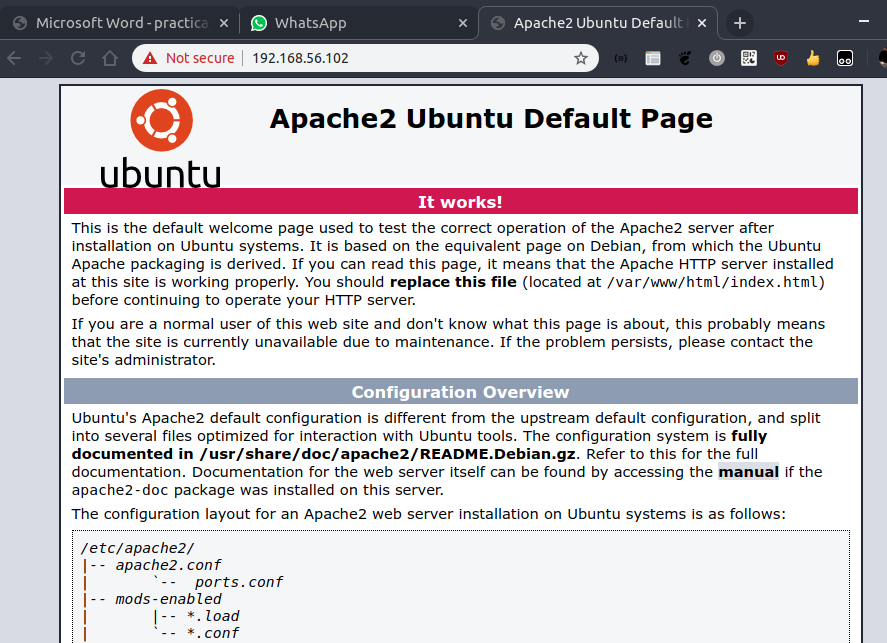
\includegraphics[scale=0.5]{6.png} 
\caption{Certificado inválido}
\end{figure}

\begin{figure}[H]
\center
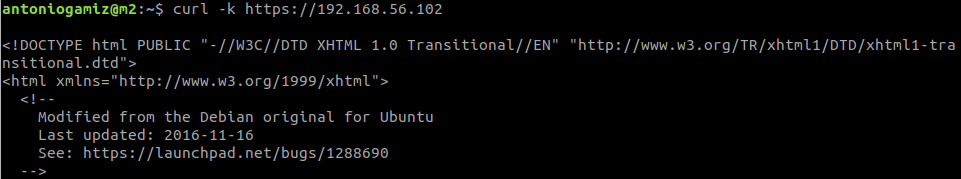
\includegraphics[scale=0.5]{7.png}
\caption{No funciona sin -k}
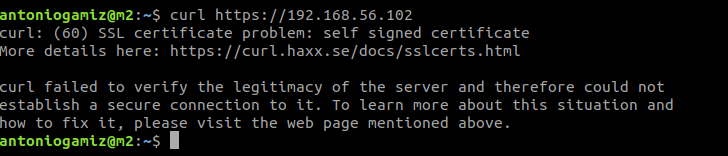
\includegraphics[scale=0.5]{8.png}
\caption{Functiona con la opción -k}
\end{figure}

Pasamos los certificados a \textit{M2}:

\begin{figure}[H]
\center
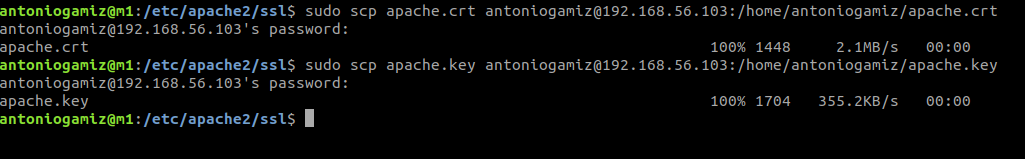
\includegraphics[scale=0.5]{9.png}
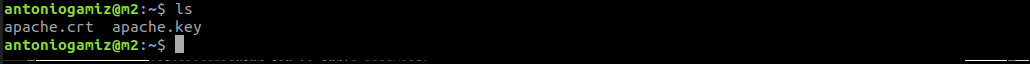
\includegraphics[scale=0.5]{10.png}
\end{figure}

Repetimos los pasos hechos anteriormente:

\begin{figure}[H]
\center
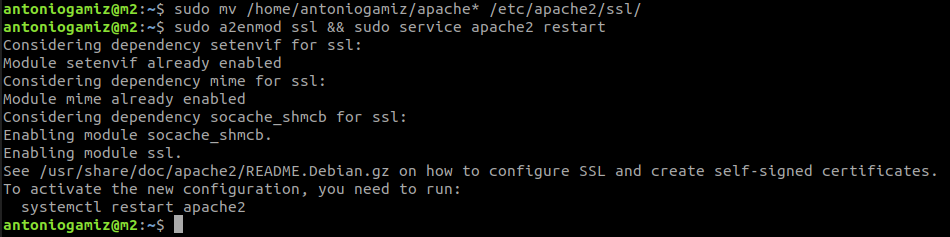
\includegraphics[scale=0.5]{11.png}
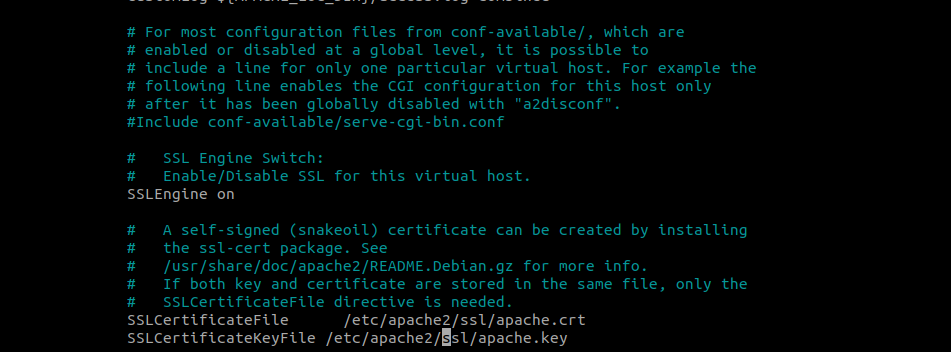
\includegraphics[scale=0.5]{12.png}
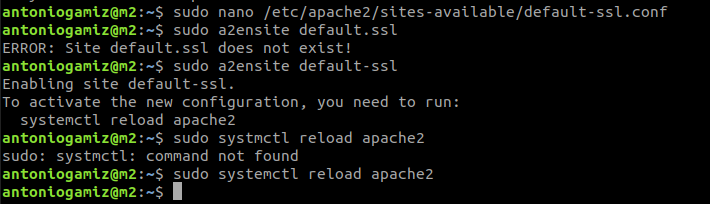
\includegraphics[scale=0.5]{13.png}
\end{figure}

Cambiamos la configuración de \textit{nginx} en \textit{M3}:

\begin{figure}[H]
\center
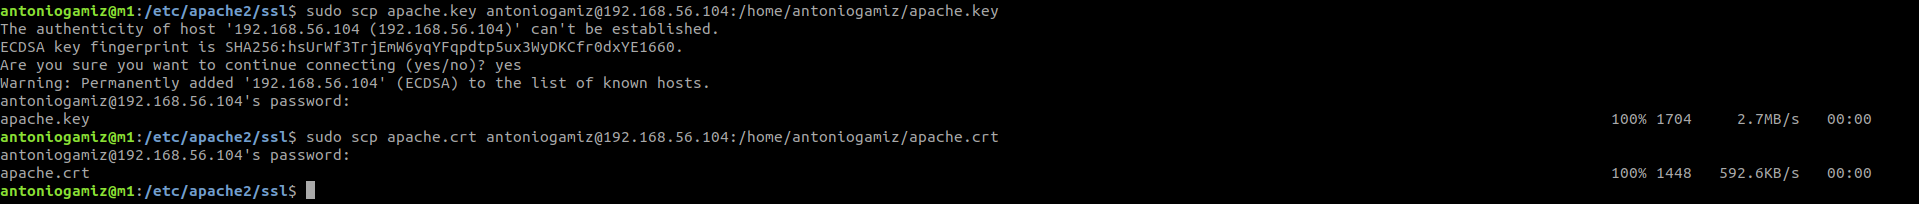
\includegraphics[scale=0.4,width=\textwidth]{14.png}
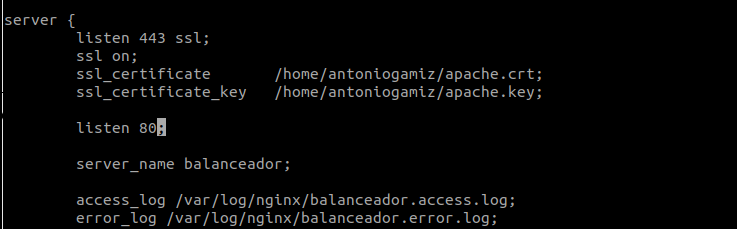
\includegraphics[scale=0.5]{15.png}
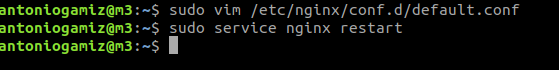
\includegraphics[scale=0.5]{16.png}
\end{figure}

\section{Configuración del cortafuegos}

Una vez configurados los certificados en ambas máquinas, pasamos a configurar el cortafuegos. Creamos la configuración deseada en un script:

\begin{figure}[H]
\center
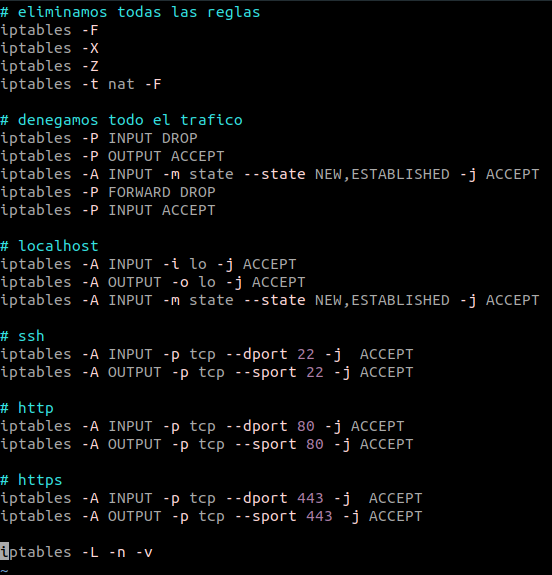
\includegraphics[scale=0.5]{18.png}
\end{figure}

La aplicamos en \textit{M1}:

\begin{figure}[H]
\center
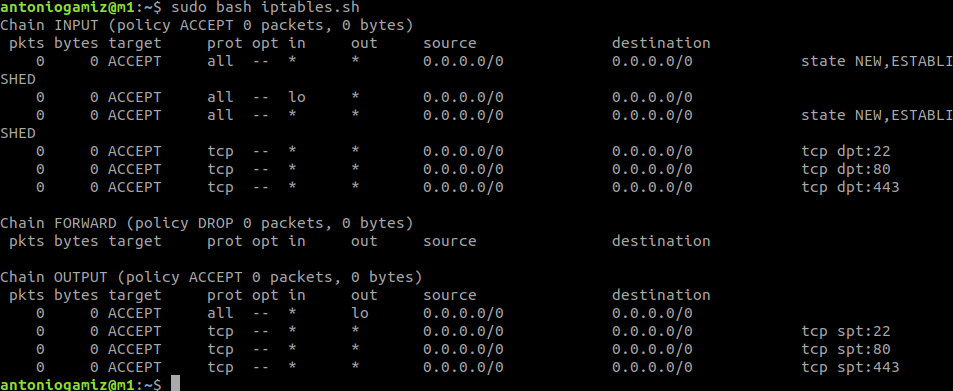
\includegraphics[scale=0.3,width=\textwidth]{17.png}
\end{figure}

Pasamos el archivo a \textit{M2} y lo aplicamos también:

\begin{figure}[H]
\center
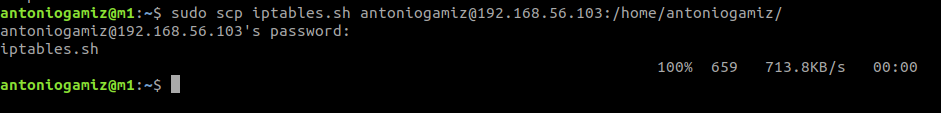
\includegraphics[scale=0.5,width=\textwidth]{19.png}
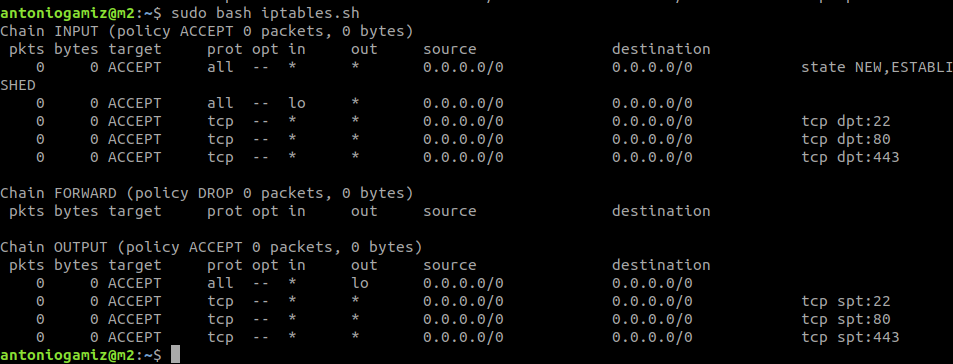
\includegraphics[scale=0.5,width=\textwidth]{20.png}
\end{figure}

Comprobamos que el balanceador sigue funcionando:

\begin{figure}[H]
\center
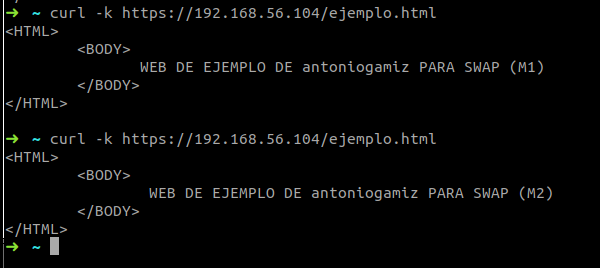
\includegraphics[scale=0.5,width=\textwidth]{21.png}
\end{figure}

\section{Segunda tarea opcional}

Al igual que antes, creamos las configuraciones necesarias en un script, uno para \textit{M1} y \textit{M2}, y otro para \textit{M3}. \textit{M3} solo debe aceptar conexiones \textit{http} y \textit{https} (además de \textit{ssh}), por lo que podemos usar el script anterior. Lo copiamos y lo ejecutamos:

\begin{figure}[H]
\center
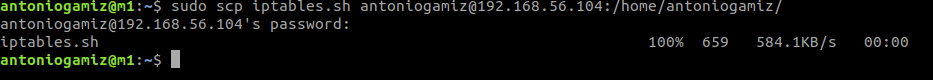
\includegraphics[scale=0.5,width=\textwidth]{22.png}
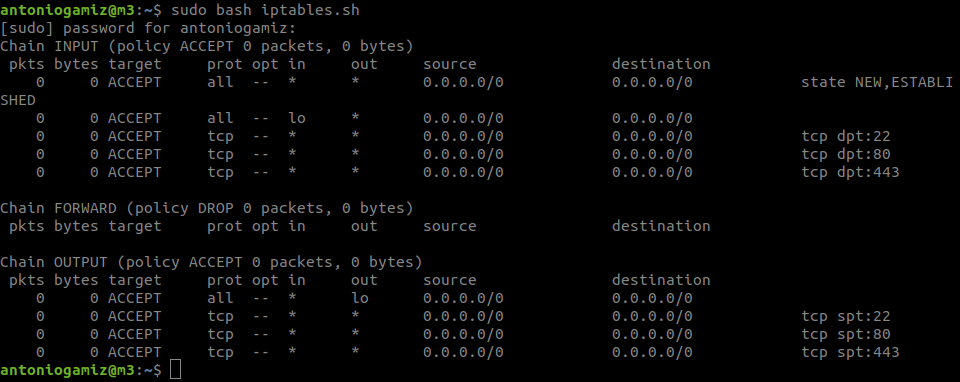
\includegraphics[scale=0.5,width=\textwidth]{23.png}
\end{figure}

Para \textit{M1} y \textit{M2} igual excepto que las conexiones sólo pueden venir desde \textit{M3}:

\begin{figure}[H]
\center
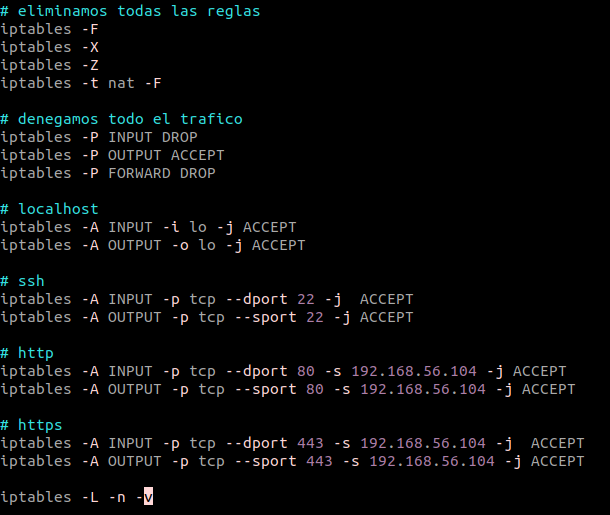
\includegraphics[scale=0.5]{26.png}
\end{figure}

Como antes, aplicamos cambios, pasamos el archivo al otro host y los aplicamos también:

\begin{figure}[H]
\center
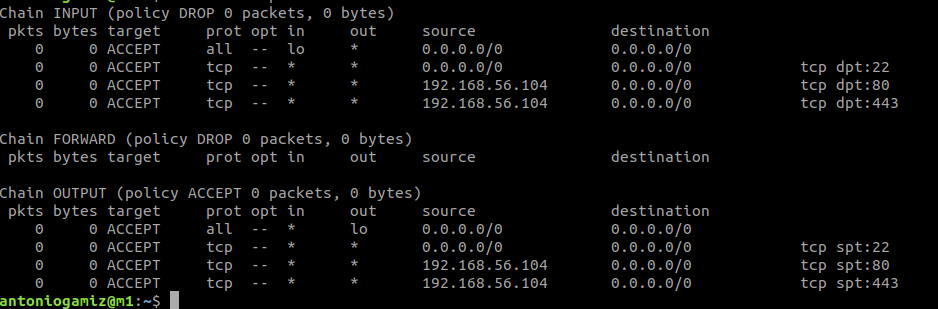
\includegraphics[scale=0.5]{27.png}
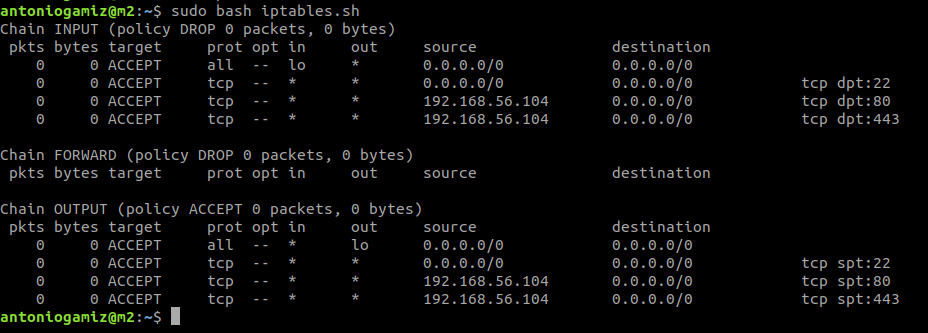
\includegraphics[scale=0.5]{28.png}
\end{figure}

Comprobamos que funciona si hacemos la petición a \textit{M3}:

\begin{figure}[H]
\center
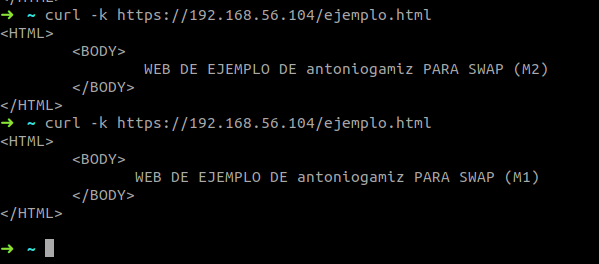
\includegraphics[scale=0.5]{29.png}
\end{figure}

Pero no funciona si accedemos directamente a \textit{M1}:

\begin{figure}[H]
\center
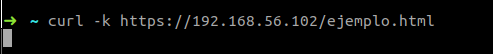
\includegraphics[scale=0.5]{30.png}
\end{figure}

Deberíamos haber usado la cláusula \textit{REJECT} para evitar llegar al timeout.

\end{document}